\documentclass[border=0mm]{standalone}

\usepackage{import}
\subimport{../../../}{preamble.tex}

\usepackage{tikz}
\usetikzlibrary{calc}
\usepackage{pgfplots}

\begin{document}

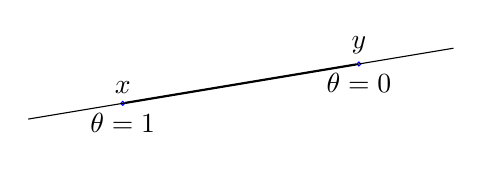
\begin{tikzpicture}
  
  \node[circle, inner sep=0.5, draw=blue] (x1) at (-1, 2) {};
  \node[circle, inner sep=0.5, draw=blue] (x2) at (2, 2.5) {};

  \node[above] at (x1) {$x$};
  \node[below] at (x1) {$\theta = 1$};
  \node[above] at (x2) {$y$};
  \node[below] at (x2) {$\theta = 0$};
  
  \draw[thick] (x1)--(x2);
  \draw ($1.4*(x1) + {1-1.4}*(x2)$)--($-0.4*(x1) + {1--0.4}*(x2)$);
\end{tikzpicture}

\end{document}

%%% Local Variables:
%%% mode: latex
%%% TeX-master: t
%%% End:
